\documentclass[11pt]{article}
\usepackage[margin=0.5in]{geometry}
\usepackage[utf8]{inputenc}
\usepackage{setspace}
\setstretch{1}
\usepackage[english]{babel}
\usepackage[]{amssymb} 
%\usepackage[enable]{darkmode} 
\usepackage{amsmath, amsthm}
\usepackage{mdframed}
\usepackage{pgfplots}
\usepackage{booktabs}
\usepackage{enumitem}
\usepackage{hyperref}
\usetikzlibrary{pgfplots.fillbetween}  
\pgfplotsset{compat=1.17} 
\makeatletter
\newcommand{\tpmod}[1]{{\@displayfalse\pmod{#1}}}
\makeatother

\mdfdefinestyle{problemstyle}{
    innertopmargin=10pt,
    innerbottommargin=10pt,
    innerrightmargin=10pt,
    innerleftmargin=10pt,
    outerlinewidth=1pt,
    topline=true,
    bottomline=true,
    leftline=true,
    rightline=true
}

%custom enviroment for exercises
\newenvironment{exercise}{
    \begin{mdframed}[style=problemstyle]\textcolor{black}{}
}{
    \end{mdframed}
}


\title{TPHYS 121 Workshop Week 6}
\author{}
\date{\vspace{-15ex}}

\begin{document}
\maketitle

\section*{Module 3 Problems}

\subsection*{Exercise 7.2}
\begin{exercise}
    A weightlifter stands up at constant speed from a squatting position while
    holding a heavy barbell across his shoulders.
    \begin{enumerate}[label=\alph*]
        \item Draw an interaction diagram
        \item Identify the "system" on your interaction diagram.
        \item Draw a free-body diagram for each object in the system. Use
            dashed lines to connect members of an action/reaction pair.
    \end{enumerate}
\end{exercise}

\subsection*{Exercise 8.23}
\begin{exercise}
    While at the county fair, you decide to ride the Ferris wheel. 
    Having eaten too many candy apples and elephant ears, you find the 
    motion somewhat unpleasant. To take your mind off your stomach, you 
    wonder about the motion of the ride. You estimate the radius of the 
    big wheel to be $15m$, and you use your watch to find that each loop 
    around takes $25s$.
    \begin{enumerate}[label=\alph*]
        \item What is your speed and the magnitude of your acceleration?
        \item What is the ratio of your weight at the top of the ride to 
            your weight while standing on the ground?
        \item What is the ratio of your weight at the bottom of the ride 
            to your weight while standing on the ground?
    \end{enumerate}
\end{exercise}

\subsection*{Exercise 6.11}
\begin{exercise}
    The figure bellow shows the force acting on a $2.0kg$ object as it moves
    along the x-axis. The object is at rest at the origin at $t=0s$. What 
    is the acceleration and velocity at $t=6s?$.
\end{exercise}
\begin{figure}[ht!]
    \centering
    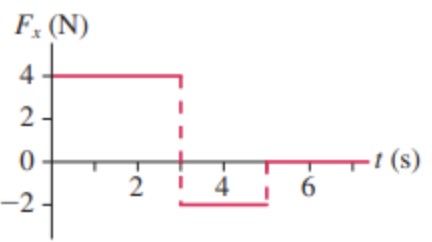
\includegraphics[width=2.5in]{images/figure6_11.png}
\end{figure}


\section*{Additional Resources}
\begin{itemize}
    \item Flipping Physics on youtube: 
        \url{https://www.youtube.com/user/flippingphysics} 
\end{itemize}

\end{document}

